\documentclass[a4paper,10pt]{article}
\usepackage[margin=3cm, nohead]{geometry}
\usepackage{natbib}
\usepackage{graphicx}
\usepackage{listings}
\usepackage{synttree}

\newcommand{\HRule}{\rule{\linewidth}{0.5mm}}

\begin{document}

\begin{titlepage}
\begin{center}

\includegraphics[width=1\textwidth]{uva}\\[1cm]

\HRule \\[0.4cm]
{ \huge \bfseries Tweedejaarsproject A.E.S.I.}\\[0.4cm]

\HRule \\[1cm]

\textsc{\LARGE  Artificial Evolution and Swarm Intelligence}\\[0.5cm]
\textsc{\Large  Verslag}\\[1cm]

\begin{tabular*}{0.95\textwidth}{@{\extracolsep{\fill}} l c r}
Jeroen \textsc{Rooijmans}	& Maarten \textsc{Inja}     & Maarten \textsc{de Waard} \\
\textsc{5887410}                &\textsc{5872464}           &\textsc{5894883}\\
\end{tabular*}

\vfill \today
\end{center}
\end{titlepage}
\tableofcontents \pagebreak

\section{Introduction}
During this project we will attempt to create a program that artificially evolves tank like agents in the RoboCode environment\footnote{RoboCode home page: http://robocode.sourceforge.net/}.
RoboCode is a simple game, where virtual tanks can fight eachother. More information and rules of the game can be found in section \ref{bi}.

It would be fairly easy to write a powerful bot ourselves, but using genetic programming\footnote{Genetic Programming wiki: http://en.wikipedia.org/wiki/Genetic\_programming} we can let a computer evolve these bots.
To test our evolved bots, we use the RoboCode environment to generate test data of battles between our evolved bots and various enemy bots. After a certain amount of battles, RoboCode generates results, these results consist of a overall score. The score is calculated using the survival rate, damage done and ranking of the previously fought battles.

There is a similar program that evolves RoboCode bots created by Klaus Meffert, the program is called RoboCode with JGAP\footnote{RoboCode with JGAP home page: http://jgap.sourceforge.net/doc/robocode/robocode.html}. After short research we found out that this program is implemented different from ours. It does not evolve on the code, like we want to, but it enables code segments, making evolving to a good bot a lot easier.

Other enemies can be bots that won online tournaments, informations and rankings of these tournaments can be found on RoboRumble\footnote{RoboRumble home page: http://robowiki.net/wiki/RoboRumble}.
The code for this project will be written in Java and available on our Google Code page \footnote{Google Code page: http://code.google.com/p/aesi/}.
We planned our activities with the Gantt chart that can be found in Appendix \ref{planning}.

\section{Project goals}
The main goal of this project is to create a Java program that evolves RoboCode bots.
These bots will evolve based on their performance, this performance needs to be tested. We use the results of multiple battles, acquired by the benchmark tool in RoboCode environment to give a bot a certain ``fitness'' score.
The evolution is done by manipulating the genotype of the bots. Therefor we need to create a representation that can manipulate the genotype and translate it to the phenotype.

\section{Method}
In order to evolve a powerfull agent using genetic programming, we first need to understand the underlying principles. This implies research on two subjects, powerful behavior in RoboCode and genetic programming.

Powerful behavior is documentated on RoboRumble, information about how to design our genetic algoritm and everything needed for that, is found in the article ``Evolving 3D Morphology and Behavior by Competition'' \cite{karlsims}.
After acquiring enough information, we will start implementing the genetic algorithm, we tried using the JGAP framework\footnote{JPAG home page: http://jgap.sourceforge.net/}, but ended up creating our own framework. More information on this is in section \ref{sec:problems}.

\subsection{Genotype}
The genotype describes a genetic constitution of the robot. The JGAP framework has predefined classes such as \textit{Chomosome}, \textit{Gen} and \textit{Population} that represent the genotype.
To implement evolutionary processes, we need to create two different representations of the genotype.

One datastructure holds information about certain method call that controls the bot.
These calls need arguments to initiate, these are also captured in the datastructure. These arguments can be mathematical formulas, control flow statements or small chunks of code that describe basic bot manoeuvres. The arguments are always doubles, which makes it easier for us.

\begin{figure}
    \centering
    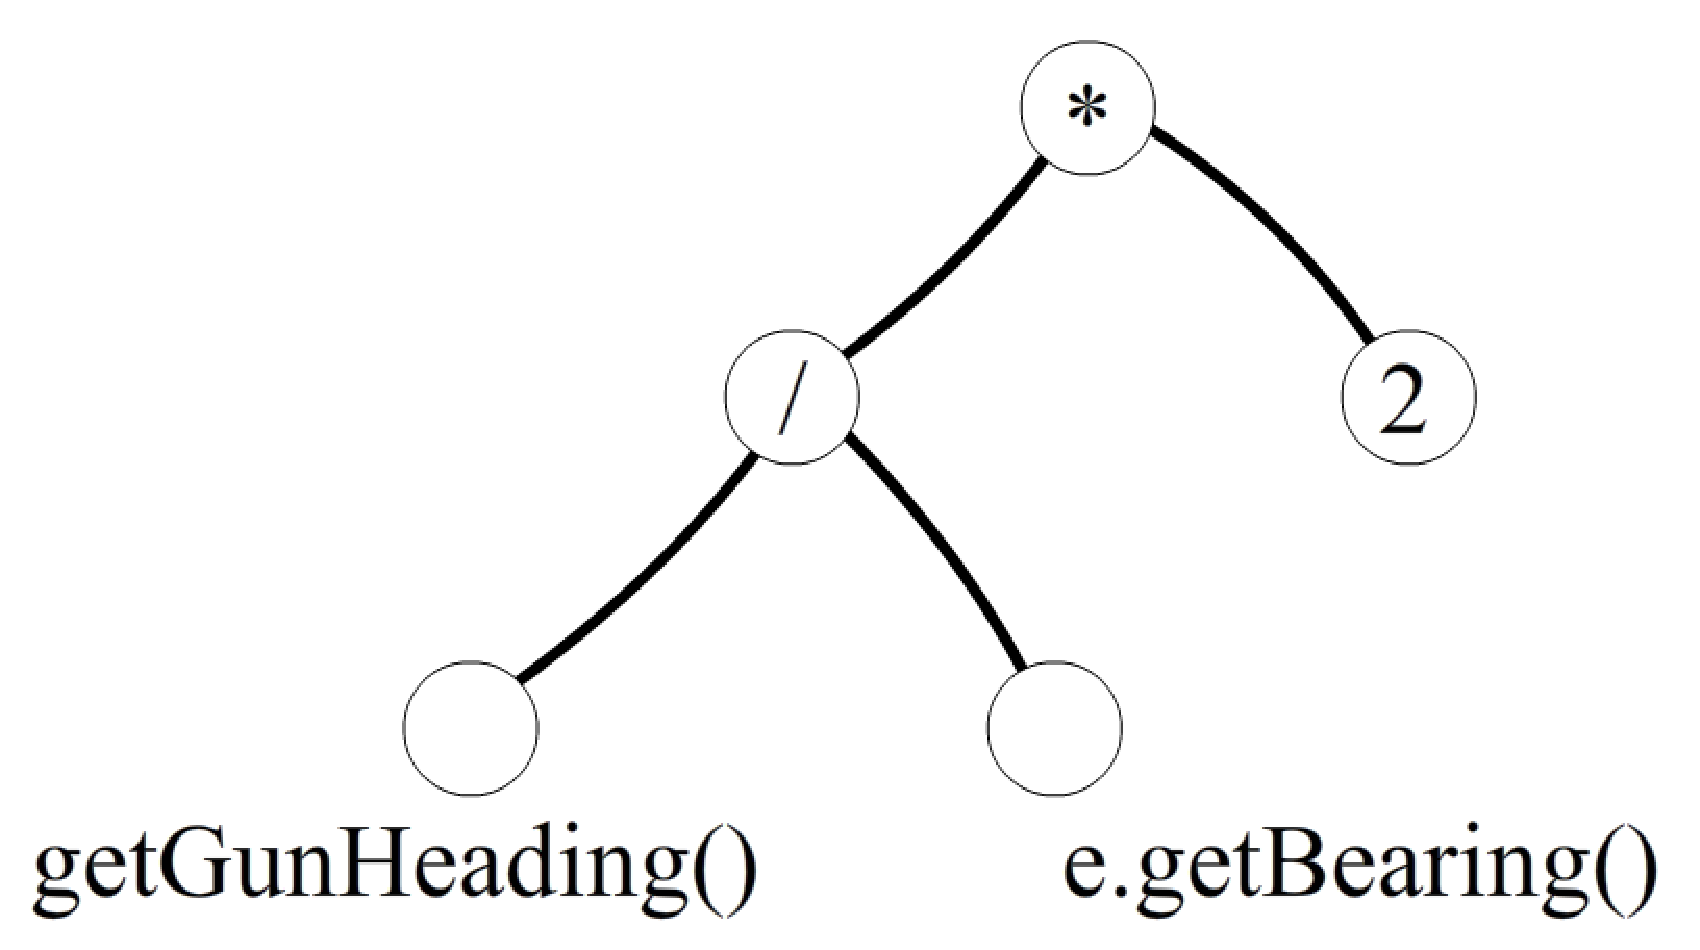
\includegraphics[scale=0.2]{tree}
    \caption{An expression tree.}
    \label{fig:tree1}
\end{figure}     

The second datastructure was needed because we value the potential of our program to evolve impressive 
mathematical functions highly. An \textit{ExpressionTree} is a binary tree holding both operators and 
values. Figure \ref{fig:tree1} shows the expression tree that represents a equation \ref{eq:tree2}. 
This representation allows us to easily mutate expressions. To add, remove or alter a node 
one only has to recursively walk down a tree to the preferred node or leaf that needs to be altered.  

\begin{equation}
    \frac{getGunHeading()}{e.getBearing()}*2
    \label{eq:tree2}
\end{equation}

These datastructures are implemented in \textit{AESIGene}. This class is based on the \textit{Gene} which is needed in the JGAP framework. We have decided that each relevant event such as \textit{onHitByBullet} or \textit{onHitWall} can be filled with Java code so each such an event represents a gene. Genes are filled with the previously mentioned datastructures and are mutated during evolution. Representing information on such a gene is currently not yet implemented but should be so in the future when we need to safe data in order to benchmark. 
 
\subsection{Phenotype}
The phenome is the resulting behaviour of the bot. Currently no real powerful behaviour has been generated. This is because not every important aspect is implemented. More of this can be found in the section \textit{result}.

\subsection{Meta language}
We need to design a meta language that creates java code from a genetic code. The genetic code is a string of digits, the location of the digit tells what gene is described, the value describes what this specific gene does. It is important to keep the genetic code meaningful and understandable so we can use the genetic code to ``see'' what kind of behaviour is evolved. This prevents our evolutional process to become a black box we use to evolve bots but where it is hard to really understand what is going on.

To properly describe how this works, we will show how java code of a simple bot, provided by RoboCode, can be represented in our genes.
This is the code of the simple bot:
\lstinputlisting[language=Java]{SpinBot.java}

This code can be described in a tree, like this:\\

\synttree[ SpinBot [ Run [ setTurnRight(10000) ] [ setMaxVelocity(5) ] [ ahead(10000) ] ] [ onScannedRobot [ fire(3) ] ] [ onHitRobot [ {if(...)} [ turnRight(10) ] ] [ isMyFault() ] ] ]

The computer will see the tree like this:\\

\synttree[ 0 [ 0 [ 12(10000) ] [ 13(5) ] [ 10(10000) ] ] [ 1 [ 3(3) ] ] [ 2 [ \#if [ 12(10) ] ] [ 4  ] ] ]

Here the upper number is an index of the gene, and the numbers on the second row are numbers indicating the index of the gene array. Under that we have array indices of the methods and their arguments, that are positioned in arrays with all the methods we can call and the arguments we can give them.


\subsection{Fitness function}
Fitness is crucial to determining the trajectory of the evolutionary process as a high fitness score will increase the chance a chromosome is transferred to the next generation of bots.

With the fitness function, we translate battle results into a appropriate fitness value. Our basic scoring measure is the fractional score F, which is computed using the score gained by our bot $S_b$ and the score gained by its adversary $S_a$ (Equation \ref{eq:ffeval1}).

Calculating the fitness score this way, we encourage our bot not only to maximize its own score, but to do so at the expense of its enemy.

\begin{equation}
F = \frac{S_p}{S_p + S_a}
    \label{eq:ffeval1}
\end{equation} \\

In early stages of the evolutionary process, bots obtain no points at all. To enhance population diversity during the initial phase of evolution we created a modified fitness function (Equation \ref{eq:ffeval2}).

\begin{equation}
F = \frac{\alpha+S_p}{\alpha+S_p + S_a}
     \label{eq:ffeval2}
\end{equation} \\

We added a small fixed constant $\alpha$. Because of this modification a bot that scores a 0 for $S_p$ but prevents his adversary to score a high $S_a$ receives a higher fitness score.

\subsection{Evolve}
Because we still need to finish some major functions we have not started evolving as of yet. We do have some results which can be found in the section \textit{results}. 

\section{Results}
Currently our program has evolved a single bot, which is capable of doing something. The results are, as discussed in previous sections, minimal, but prove promising. The robot shows action such as moving forward and rotating both it's body and gun but not yet a change in behaviour when events are caught. This means we completed the basis but need to focus on the evolutionary process that will create bots with more interesting behaviour.

We need to be able to compare our results to other bots to give the results a meaning. During this project we will create some bots ourselves and download bots that have proven to be powerfull in online tournaments. These bots will be battling against our bots. This way we can find out if the bots evolved with genetic programming can stand against human made bots. There is a paper ``GP-Robocode: Using Genetic Programming to Evolve Robocode Players'' \cite{shichel} about RoboCode bots evolved with a genetic framework that participated in a online tournament with 27 participants. Other bots were all human written. The bot (``GPBot'') ended third.

\section{Background information}
\label{bi}
\subsection{RoboCode Game}
The RoboCode game is a battle between virtual tanks. These can move around and shoot. Time is represented in ticks. There are several things happening each tick. For example the robot is allowed a certain amount of processing time to calculate and execute actions. The game world is also updated, meaning that objects are relocated according to the physical laws of the game and potential collisions between objects and the results of such collisions are calculated.

\subsection{Robot Anatomy}
\begin{figure}
\label{anatomy}
\centering
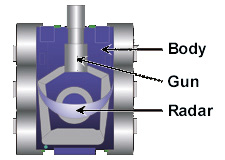
\includegraphics[scale=1.5]{anatomy.jpg}
\caption{The robot anatomy}
\end{figure}
A robot consists of three seperate parts, the radar which is mounted on the barrel which is mounted on the body. All parts can be rotated seperately. The barrel fires bullets, the radar scans for other tanks and the body drives around in the arena. This is shown in figure \ref{anatomy}.
\subsection{RoboCode rules}

The Robocode environment has specific rules constraining our bot. I will explain the basic rules of the RoboCode game and how a bot can behave.
A fight starts by placing all participating bots in the arena at random places. All bots have a certain amount of energy. Energy is lost by getting shot by an enemy or ramming walls and enemies. Certain actions also use up energy, for example shooting a bullet.

A bot can gain energy by hitting an opponent. When a bot is out of energy, it is disabled and explodes.

\subsection{Programming the Robot}
Programming a robot means \textit{extending} the robot class from RoboCode. This allows us to program methods that catch events that are launched by RoboCode (such as \textit{robotScannedEvent}) and program what we would like the robot to do in such cases (such as \textit{rotateGun}). The robots behavior relies completely on what events occur during a battle. The robots actions during a certain event is generated by the evolutionary process. 

\newpage
\section{Planning}
\subsection{Documentation}
\begin{itemize}
 \item create workplan, everybody
 \item round of halfway report and presentation, M. de Waard
 \item present halfway presentation, everybody
 \item finish end report and presentation, J. Rooijmans
 \item present final product, everybody
 \item maintain documentation, M. Inja
\end{itemize}

\subsection{Initiation}
\begin{itemize}
\item create planning and set up websites, M. Inja
\item present workplan, everybody
\item familarization with programs, M. Inja, M. de Waard
\item read articles about genetic algoritms, J. Rooijmans
\end{itemize}

\subsection{Genetic programming, single bots}
\begin{itemize}
\item create genotype, J. Rooijmans
\item create fitness function, M. de Waard
\item evolve, M. Inja
\end{itemize}

\subsection{Test phase}
\begin{itemize}
\item benchmark with RoboResearch, M. de Waard
\item compare RoboCode with JPAG, M. Inja
\item design and compare with own bot, everybody
\item compare with bots from the internet, J. Rooijmans
\end{itemize}

\subsection{Genetic programming, teams}
\begin{itemize}
\item create genotype, J. Rooijmans
\item create fitness function, M. de Waard
\item evolve, M. Inja
\item benchmark, everybody
\end{itemize}
\newpage
\bibliographystyle{abbrv}
\bibliography{ref}
\newpage
\appendix
\section{Planning}
\label{planning}
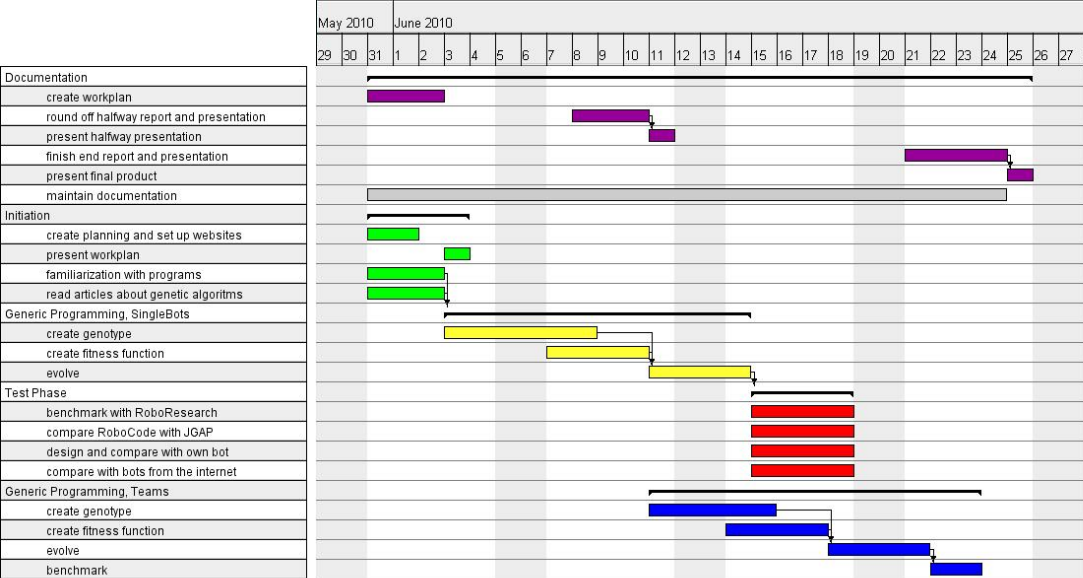
\includegraphics[height=0.75\textwidth, angle=-90]{planning.png}
\end{document}
